\section{Crawler}
A crawler was implemented that visits other nodes and request the full chain of that node.
The crawler was used for the experiments and
is a first step in a more sophisticated crawler that will help to solve the known vulnerabilities.
These vulnerabilities will be described in chapter \ref{problems}.

\subsection{Recursively request blocks}
Dispersy provides a list of other nodes that were recently found
and can report when the node itself is found by an other node.
Both are sources of destinations nodes that the crawler will visit
and request the chain from.

The crawler will first request from a node the block with sequence number $-1$.
This denotes that he wants the latest block in his chain.
The node returns this block to the crawler.
The crawler will persist the block if it is not yet know.

The newly retrieved block is chained to two blocks with the previous hashes.
The crawler will check if these blocks are present in the database.
If any block is not present,
then the crawler will request that particulair block if the node is known in Dispersy.
If the node is not known, the block is ignored.
This is done recursively untill the crawler reaches the genesis block of the chain.
In this fashion a breadth first search is implemented for any unknown block
that is chained in chronologically before the latest block.

\begin{figure}
	\centerline{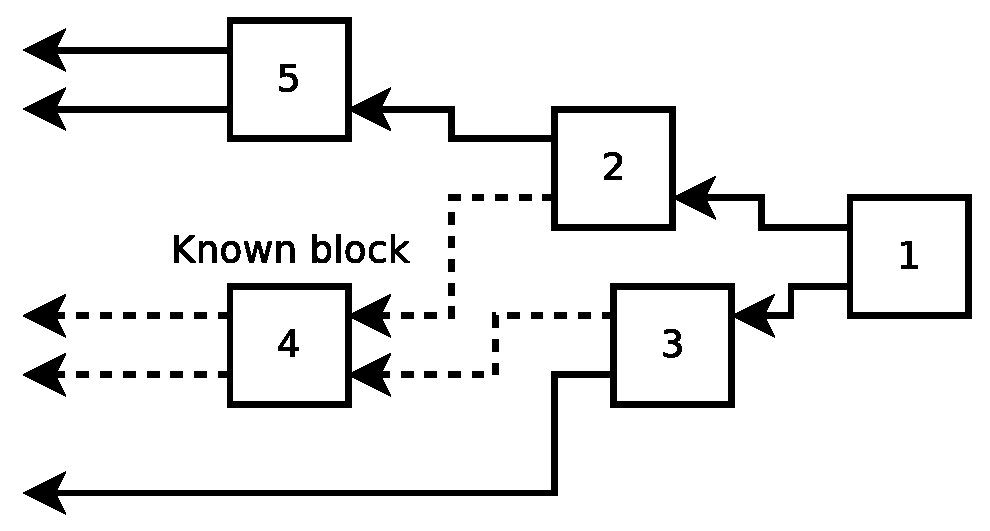
\includegraphics[scale=0.3]{design/figs/crawler.eps}}
	\caption{Example of the crawler looking for unknown blocks.}
	\label{fig:crawler-example}
\end{figure}

An example can be seen in Figure \ref{fig:crawler-example}.
In this example the line arrows denote paths that the crawler follows
and dotted lines are paths that the crawler ignores.
Block 4 is already known by the crawler.
Block 1 is retrieved by the crawler and the crawler sees hash links to block 2 and 3.
These are retrieved and the block finds links to block 4 and 5.
Because block 4 is already known, block 4 is ignored.
Only block 5 is retrieved.
The crawler follows the links further outside the displayed example.

\subsection{Improvements}
The crawler is a first, simple step towards a more sophisticated crawler.
Tribler has implemented already more sophisticated crawlers for Bartercast
and these techniques can be reused for the MultiChain crawler.
For example bloom filters can be used in conjunction with the knowledge
that every record is a part of the chain to quickly request multiple blocks\cite{broder-bloomfilter}\cite{logiotatidis-splash}.
Blocks could also be send in a more efficient way by sending multiple blocks per message.
Lastly an obvious improvement is to also crawl and retrieve blocks from other nodes present in a node.
This is currently not yet implemented.


